% !TeX program = pdflatex
% !BIB program = biber



\section{Portability}
\label{sec:Portability}

\subsection{Clean Code/Semantic Coding: Separating Content and Formatting}

All written texts are structured into words and sentences. If they are long enough, texts are also structured into paragraphs. Academic texts, in addition, feature sections, subsections, and often subsubsections, as well as figures, tables, lists of references, and potentially appendices. These structural elements are associated with headings\slash titles and captions.

The structure of a~document is conveyed to the reader through \emph{formatting}. Effective formatting of academic documents, thus, requires that all elements of a~particular type---say, section headings---be identifiable as such. Identifiability is achieved through styling that is \emph{consistent within type} and \emph{distinct across types}. For example, all section headings must be formatted identically, and at the same time, they must look different from subsection headings.

As a~consequence, one should refrain from using manual, discretionary formatting whenever possible. In line with this principle, the source code of this template refers to the document's structure as much as possible. This is also called ``semantic coding'': using code that describes the \emph{meaning} of the content and not \emph{how} those elements should look.
\begin{itemize}
	\item Examples for \emph{semantic} commands are \verb|\author|, \verb|\title|, \verb|\section|,  \verb|\emph|, \verb|\url|, \verb|\cite|, \verb|\begin{figure}| \textellipsis\ \verb|\end{figure}|, \verb|\caption|, \verb|\begin{quote}| \textellipsis\ \verb|\end{quote}|.
	\item Examples for LaTeX commands that are \emph{not semantic}---and should be avoided---are \verb|\textbf|, \verb|\textit|, \verb|\newpage|, \verb|\pagebreak|, \verb|\linebreak|, \verb|\\|, \verb|\noindent|, \verb|\smallskip|, \verb|\centering|, \verb|\noindent|, \verb|\hspace|, \verb|\vspace|, \verb|\cellcolor|, \verb|\multirow|.
\end{itemize}

The reason why one should stick to using semantic commands is that they keep the code \emph{portable}: Semantic code can be \emph{reused} across document without any changes (or at least without major adjustments). This is not then case with nonsemantic code, that is, code that includes manual formatting instructions. Instructions like \verb|\bigskip|, \verb|\hspace|, \verb|\\| (even worse, \verb|\\ \\|), etc. may result in decent formatting in a~particular document but are bound to lead to undesirable formatting in another document. This applies, in particular, when you face the task of combining several research papers into one, ``cumulative'' doctoral thesis. Moreover, manual formatting is error-prone, as it easily leads to inconsistent styling.

This entails two things: First, the formatting should be determined, as much as possible, in the \emph{preamble} of the LaTeX document. This comes at the cost, of course, of a~rather long preamble. Second, instead of defining custom commands, one should \emph{redefine} standard LaTeX commands or use (widely adopted) packages that are available on \caps{CTAN} (\url{https://ctan.org}).

This template follows the above principles, resulting in clean, portable code: The source code of the body of this template (apart from the boxes with examples) consists almost completely of semantic, basic LaTeX, with commands from popular packages on top.

\subsection{Using BibLaTeX (Rather Than BibTeX)}

This template uses the modern BibLaTeX framework (the \textit{biblatex-chicago} package, \url{https://ctan.org/pkg/biblatex-chicago}, to be precise) instead of the vintage BibTeX framework to manage the references included in the document. The reason for this choice is that BibLaTeX is much more flexible than BibTeX and also handles multi-language references much better.

Moreover, in line with the principle describe above, BibLaTeX permits much better separation of a~document's content (in this case, the \textit{.bib} file) and its formatting (of the citations and the bibliography) than BibTeX. In particular, suppressing output of information that is present in a~\textit{.bib} file is cumbersome with BibTeX: It amounts to editing the ``bibliography style'' \textit{.bst} file, and \textit{.bst} files have a~syntax that is completely different from LaTeX and difficult to learn. It is usually easier to just remove the information from the \textit{.bib} file. This, however, impacts the portability of the \textit{.bib} file: In other circumstances one might want that very information to be present. BibLaTeX simplifies skipping information that is present in the \textit{.bib} file.

An example: Researchers frequently present their research in the form of posters. Space on posters is usually quite limited. Hence, one might not want authors' first names to be abbreviated on a~poster. In the associated paper, however, the names should be printed in full to minimize ambiguity. With BibTeX, this requires time-consuming adjustments of the \textit{.bst} file. With BibLaTeX, it is much easier: In the \textit{.tex} file for the poster, one can include the command
\begin{quote}
	\verb|\ExecuteBibliographyOptions{giveninits = true}|
\end{quote}

Similarly, in a~paper, the list of references should include \caps{URL}s or \caps{DOI}s (digital object identifiers) whenever they exist, to make it easy for readers to locate a~cited work. On a~poster, by contrast, one might want to suppress \caps{DOI}s and \caps{URL}s. With BibTeX, this would require time-consuming adjustments of the \textit{.bst} file. With BibLaTeX, one can simply do, for instance,
\begin{quote}
\begin{verbatim}
\AtEveryBibitem{%
  \ifentrytype{article}{\clearfield{doi}\clearfield{url}}{}%
}
\end{verbatim}
\end{quote}

Using BibLaTeX requires using the program \verb|biber| instead of \verb|bibtex| for compiling the bibliography. When using the Overleaf online service, using \verb|biber| instead of \verb|bibtex| is as simple as it gets: Overleaf automatically chooses \verb|biber| to compile the bibliography when it encounters BibLaTeX's \verb|backend = biber| option.\footnote{This applies to the commercial version (\url{https://www.overleaf.com}) as well as to free versions \url{https://overleaf-students.astro.uni-bonn.de/} and \url{https://uni-bonn.sciebo.de/apps/overleaf_nextcloud/launcher/launch}.} And when using the TeXstudio editor (\url{https://texstudio.org}), an easy way to make this happen is to include the ``magic comment''
\begin{quote}
	\verb|% !BIB program = biber|
\end{quote}
at the beginning of the \textit{.tex} file.

\subsection{Using the \mbox{\textit{tabularray}} Package (Rather Than \mbox{\textit{tabularx}}\slash \mbox{\textit{tabulary}}\slash \mbox{\textit{tabu}}, \mbox{\textit{booktabs}}, \mbox{\textit{longtable}}, \mbox{\textit{xltabular}}, \mbox{\textit{multirow}}, \mbox{\textit{makecell}}, \mbox{\textit{colortbl}}, \mbox{\textit{parnotes}}, \mbox{\textit{threeparttable}}, \textellipsis\!)}

The principle of separating the content from its formatting as much as possible can also be applied to tables. The \mbox{\textit{tabularray}} package (\url{https://ctan.org/pkg/tabularray}) allows you to do just that. \mbox{\textit{tabularray}} has been around since May 2021, so it is relatively new---but it has already matured into a~package that is extremely useful. \mbox{\textit{tabularray}} replaces (or loads) all the other table-related LaTeX packages that you may have used so far---like \mbox{\textit{tabularx}}\slash\mbox{\textit{tabulary}}\slash\mbox{\textit{tabu}}, \mbox{\textit{longtable}}, \mbox{\textit{xltabular}}, \mbox{\textit{multirow}}, \mbox{\textit{makecell}}, \mbox{\textit{booktabs}}, \mbox{\textit{colortbl}}, \mbox{\textit{parnotes}}, \mbox{\textit{threeparttable}}, \textellipsis

Separating the contents of a~table from its formatting means that no formatting instructions whatsoever need to be placed in the table cells---neither for drawing rules between table rows nor for highlighting entries nor for increasing spacing nor for changing alignment, and so on. Instead, the placement of rules at the top and bottom of a~table or between particular rows, the specification of column widths, the specification of font sizes and cell alignment, desired highlighting via boldface or a~background color, etc., can all be coded as arguments to the table environment. This is beneficial in at least three aspects:
\begin{itemize}
	\item The source code of the table's contents is very clean. This particularly applies to animated Beamer presentations: no need to put \verb|\pause|\slash \verb|\only|\slash \verb|\cellcolor|\slash\textellipsis in table cells.
	\item  It makes table contents \emph{portable}: A~table's contents can be reused easily across multiple documents that are formatted in different ways.
	\item  It also drastically simplifies the inclusion of table contents that are produced by an external program such as Python, R, or Stata.
\end{itemize}

Further additional helpful features of \mbox{\textit{tabularray}} are:
\begin{itemize}
	\item \mbox{\textit{tabularray}} makes it easy to bottom-align or top-align particular table rows or individual cells entries, while keeping a~different alignment for the other rows\slash cells.
	\item Table entries that consist of multiple lines of text become easy to produce: Just enclose them in curly braces, like in this example: \verb|... & {Line 1 \\ Line 2} & ... \\|. No~need to use \verb|\multirow| or \verb|\makecell| any more.
	\item You can set document-wide formatting defaults to achieve consistent formatting of all tables. For instance, you can set defaults such that all tables feature the same top and bottom rules. Or, you could make all column heads be typeset in boldface document-wide.
\end{itemize}

When using \verb|\UseTblrLibrary{siunitx}|, \mbox{\textit{tabularray}} loads the \mbox{\textit{siunitx}} package. This is another useful package which permits separating content from formatting. In particular, the \verb|S|~column type is able to round numbers to a~specified precision. This means that one can include table content produced by an external program with as many decimal digits as that program produces and have LaTeX take care of the rounding.


\section{Methods}
\label{sec:Methods}

\subsection{Structuring Introduction and Discussion: Funnel and Reverse Funnel}

A~general structure that can be found in many research papers is the so-called X-shaped or ``hourglass'' structure.\footnote{See \url{https://skillsearthsciences.sites.uu.nl/writing/structure/\#attachment_2387}, Fig.\,1, and \url{https://pmc.ncbi.nlm.nih.gov/articles/PMC5405644/pdf/JHRS-10-3.pdf}, Figure~1.} This structure is brought about when the so-called ``funnel'' technique is used to write the introduction,\footnote{See  \url{https://read.aupress.ca/read/read-think-write/section/9e945e9b-62cf-4dbb-b8cd-823549ede292\#fig1401}, Figure~14.1, and \url{https://kib.ki.se/en/write-cite/academic-writing/structure-academic-texts}} and when a~``reverse funnel'' or ``upside-down funnel'' is used to write the discussion\slash concluding section:\footnote{See \url{https://read.aupress.ca/read/read-think-write/section/9e945e9b-62cf-4dbb-b8cd-823549ede292\#fig1402}, Figure~14.2, and \url{https://kib.ki.se/en/write-cite/academic-writing/writing-conclusion}.}
\begin{enumerate}
	\item The paper starts with a~\emph{broad} perspective at the beginning of the introduction, which becomes \emph{narrower} with every sentence, leading to the paper's narrow research question.
	\item The \emph{narrowest} part is when the exact research question is posed, the research methodology is described in detail, and the results are derived\slash presented.
	\item When the results are discussed and related to the literature in the concluding section, the perspective becomes \emph{broad} again.
\end{enumerate}

An example of the ``funnel'' technique can be found in \autoref{fig:sigfridsson:intro}, and of the ``reverse funnel'' technique in \autoref{fig:sigfridsson:conclusion}.

\begingroup

\SetTblrInner[tblr]{
	colspec = {X[1.9] X[l]},
	column{1} = {
		bg = UBonnBlue!5, font = \rmfamily\small, leftsep = 3ex,
	},
	column{2} = {
		bg = UBonnBlue!5, font = \sffamily\footnotesize\setlength{\baselineskip}{2.75ex}\RaggedRight, rightsep = 3ex
	},
	hborder{1-Z} = {abovespace = 0pt, belowspace = 0pt},
	hborder{1} = {belowspace = 2.25ex},
	hborder{Z} = {abovespace = 2.25ex},
	hline{1-Z} = {0pt},
	vborder{2} = {rightspace+ = 0.5em},
	width = \linewidth,
}

\begin{figure}[p]
	\begin{tblr}{}
		Molecular simulation methods have become an important technique in many areas of chemistry through the recent advent of effective and wide-spread software for molecular mechanics, molecular dynamics, and Monte Carlo simulations, and procedures for the estimation of free energy differences. In all such methods, a~proper description of the electrostatic interactions within the simulated system is of key importance, \textellipsis\ However, in most implementations, \textellipsis, the simplest possible solution is used, \textellipsis\ Thus, most classical simulation methods need a~point-charge parameterisation of the molecules of interest.
		&
		{%
			\textit{Paragraph~1} \\
			\textmd{Broad introduction with general description of the research field (``many areas of
			chemistry''), research topic (``molecular simulation methods''), and recent development (``through the recent advent of \textellipsis''). Followed by a~more detailed description of crucial aspects in this context (``In all such methods, a~proper description \textellipsis\ is of key importance'') and of shortcomings of existing methods.}
		}
		\\
		\hspace{\baselineskip}Unfortunately, atomic charges are not observables, i.e. they cannot unambiguously be determined by experiments or quantum chemical calculations. Therefore, a~large number of methods have been suggested for the estimation of point charges [1]. Several groups have tried to derive the charges directly from experimental quantities, \textellipsis\ Yet, relevant data is usually missing or too scarce to allow a determination of all charges in interesting molecules. Instead, most techniques derive atomic charges from quantum chemical calculations.
		&
		{%
			\textit{Paragraph~2} \\
			Narrowing down the topic: Description of the state of the art and of issues and limitations observed in the literature.%
		}
		\\
		{%
			\hspace{\baselineskip}The simplest way to determine quantum chemical charges is the Mulliken population
			analysis. \textellipsis\ Although, Mulliken charges are known to strongly depend on the basis set [6] and to reproduce electrostatic moments poorly [1], they are still widely used due to their simplicity. Several other \textellipsis\ methods have been devised to cure the problems of the Mulliken charges [1], \textellipsis
			\\
			\null\hspace{\baselineskip}\textellipsis
		}
		&
		{%
			\textit{Paragraph 3} \\
			Further description of the state of the art: strengths and weaknesses of existing approaches. \\
			\strut \\[2ex]
			\textit{Paragraphs 4--6} \\
			Further description of unresolved issues.
		}
		\\
		\hspace{\baselineskip}In this paper, we make a critical analysis of the four most popular potential-based point-charge methods, \textellipsis\ It is shown that these methods may give widely different results and possible explanations for this are discussed. Two alternative methods for deriving atomic charges are suggested, which avoid the arbitrariness in the selection of potential points, and their performance is judged using \textellipsis
		&
		{%
			\textit{Paragraph~7} \\
			Narrow description of the specific contribution of this paper: Identification of undesirable arbitrary variation in simulation results of existing methods, which inspired development of an ``alternative methods'' that avoids this issue.
		}
	\end{tblr}%
	\caption{%
		Illustration of the funneling approach, using the ``Introduction'' section from \citet{sigfridsson}.
	}
	\label{fig:sigfridsson:intro}
	\begin{figurenotes}
		The full text of the article by \citet{sigfridsson} is available at \url{https://lucris.lub.lu.se/ws/portalfiles/portal/135489685/25_charges.pdf}.
	\end{figurenotes}
\end{figure}


\begin{figure}[p]
	\begin{tblr}{}
		Potential-based charges strongly depend on the way the potential points are selected. We have presented and tested a~new method that avoids such a~dependence, \caps{CHELMO}. It fits the charges directly to the electrostatic moments and it performs as well, or better, as the best electrostatic potential method judging from the calculated electrostatic potential and moments. \textellipsis\ The major disadvantage of the method is that it cannot be used for large molecules, since there is a~limited number of moments. No more than 25~independent charges in a~molecule can be determined if all moments up to hexadecapole moments are used. In practice it should not be used for molecules with more than about 20 atoms since otherwise the higher moments may be poorly reproduced \textellipsis\ This could be remedied if moments higher than hexadecapole moments are calculated but such moments are not included in the output of normal quantum chemical packages.
		&
		{%
			\textit{Paragraph~1} \\
			Narrow recap of the first contribution of the paper: brief description of the issue and how it was solved by the new method. Followed by description of the limitations of the new method. Outlook how these limitations could be overcome.
		}
		\\
		\hspace{\baselineskip}In order to get a~method that can be used for larger system, we constructed the \caps{CHELP-BOW} method, which estimates the charges from a Boltzmann-weighted fit to the electrostatic potential. It has the advantage over the other \textellipsis\ methods that \textellipsis\ The present implementation of the \caps{CHELP-BOW} method is very simplified, but in a future publication we will refine and thoroughly test the method. However, the results are conclusive enough to show that the method \textellipsis\ has the desired behaviour. \textellipsis\ Clearly, this is the method we recommend for general use.
		&
		{%
			\textit{Paragraph~2} \\
			Narrow recap of the central contribution of the paper and how it relates to the literature: how existing methods were further improved upon by the second method proposed in this paper. Followed by outlook on future advances and recommendation for researchers in the field.
		}
		\\
		\hspace{\baselineskip}An important advantage of the methods developed in this paper is that they are general, i.e. they can be used with any quantum chemical program and they can use experimental data (\textellipsis\!) as well. The only thing that has to be changed is the input section of the programs. Thus any quantum chemical basis sets can be used, and any level of theory that gives a~wave function may be employed. Furthermore, the methods can easily be adapted to \textellipsis
		&
		{%
			\textit{Paragraph~3} \\
			Broader implications due to the generality of the new method.
		}
		\\
		\hspace{\baselineskip}Finally, a comment on the traditional electrostatic potential methods. \textellipsis\ Thus, we cannot see any justification to use \caps{CHELP} charges except for backward comparisons.
		&
		{%
			\textit{Paragraph~4} \\
			Other broader implications.
		}
	\end{tblr}%
	\caption{%
		Illustration of the ``reverse funneling'' approach, using the ``Concluding Remarks'' subsection from \citet{sigfridsson}.
	}
	\label{fig:sigfridsson:conclusion}
\end{figure}

\endgroup

\subsection{Some Questions That May Help You Guide Writing Your Paper}

You may find the following list of questions helpful as a~guide to making sure that your manu\-script covers all important aspects. The questions are primarily intended for doctoral and advanced researchers, but they may also be helpful to students writing term papers and theses.

Your introduction might answer the following questions (not necessarily in this order, but this order will give rise to a~``funnel'' structure):
\begin{enumerate}[labelindent = \parindent, leftmargin = 2\parindent]
	\item What do we already know?
	\item What do we not know yet (the ``knowledge gap'')?
	\item Why is it interesting\slash relevant to close the gap?
	\item \emph{What is the research question? [R]}
	\item Why is it interesting to answer the research question?
	\item How do we contribute to closing the knowledge gap: How do we answer the research question? (Which method do we use?)
	\item Why is the chosen method (more) suitable (than alternative methods) for answering the research question?
\end{enumerate}

And your conclusion/discussion might answer the following questions (again, not necessarily in this order, but this order will give rise to a~``reverse funnel'' structure):
\begin{enumerate}[resume, labelindent = \parindent, leftmargin = 2\parindent]
	\item What was the knowledge gap before the current study? [Similar to the introduction.]
	\item \emph{How did we contribute to closing that gap, and what did we find? [A]} (Which method\slash dataset did we use, and what are the results?---Recap and take-home message.)
	\item How do our results relate to (confirm\slash contradict\slash complement\slash extend) the results from previous and other contemporaneous studies?
	\item What part of the gap is still open? (Phrased a~bit more negatively: What are the limitations of our approach?)
	\item Next steps\slash avenues for future research: How could we go about closing the remaining knowledge gap (by removing the limitations of our current approach)?\footnote{John Cochrane might do away with question~12. See his ``Writing Tips for Ph.D. Students,'' \url{https://www.fma.org/assets/docs/membercontent/writing_cochrane.pdf}.}
\end{enumerate}

In her book \textit{The Little Book of Research Writing},\footnote{For a quick summary of the book, see \url{https://mauve-porcupine-8992.squarespace.com/s/Chaubey_Research_Writing-bxdd.pdf}. See also \url{https://www.econscribe.org/about} and \url{https://arxiv.org/pdf/2012.07787}.} Varanya Chaubey proposes a~simpler list of only three items---the ``RAP method'':
\begin{itemize}
	\item The ``R'' stands for ``research question.''
	\item The ``A'' stands for ``answer'' (to the research question, of course).
	\item The ``P'' stands for ``positioning statement.'' (How does our manuscript relate to the literature: Does it corroborate or extend or contradict others' findings?)
\end{itemize}

Relating the ``RAP'' approach to the the list of questions above, question~4 is the~``R,'' the answer to question~9 is the~``A,'' and the remaining questions spell out the~``P.''

\subsection{Structuring Paragraphs in Academic Manuscripts}

\begingroup

\setul{0.3ex}{0.5ex}

\SetTblrTemplate{contfoot}{empty}
\SetTblrTemplate{conthead}{empty}
\SetTblrOuter[longtblr]{
	entry = none,
	label = none,
	postsep = 0.75\newbaselineskip plus 10ex,
	presep = 0.75\newbaselineskip plus 10ex,
}
\SetTblrInner[longtblr]{
	colspec = {X[2.15] X[l]},
	column{1} = {
		bg = UBonnBlue!5, font = \rmfamily\small, leftsep = 3ex
	},
	column{2} = {
		bg = UBonnBlue!5, font = \sffamily\bfseries\footnotesize\setlength{\baselineskip}{2.75ex}, rightsep = 3ex
	},
	hborder{1-Z} = {abovespace = 0pt, belowspace = 0pt},
	hborder{1} = {belowspace = 2.25ex},
	hborder{Z} = {abovespace = 2.25ex},
	hline{1-Z} = {0pt},
	vborder{2} = {rightspace+ = 0.75em},
	width = \linewidth,
}

Obviously, there is no single ``right'' way of constructing paragraphs. However, a~few basic rules can help you write paragraphs that are \emph{easy to comprehend} by your readers. A~common approach is to compose sentences such that they reflect the following functional sequence:\footnote{See \url{https://libguides.newcastle.edu.au/writing-paragraphs/structure}, \url{https://www.une.edu.au/library/students/academic-writing/write-paragraphs/paragraphs/Academic-paragraphs_v2.pdf}, \url{https://learningessentials.auckland.ac.nz/writing-effectively/paragraph/}}
\begin{enumerate}
	\item \emph{topic sentence (\caps{TS})}---which, if necessary, connects to the previous paragraph;
	\item \emph{supporting sentences (\caps{SS})}---which elaborate on the topic sentence; and
	\item \emph{concluding sentence or connecting sentence (\caps{CS})}---which refers back to the topic sentence and\slash or provides a~link to the subsequent paragraph.
\end{enumerate}

There are various ways in which the supporting sentences can be filled with content. The University of Sheffield suggests\footnote{See \url{https://sheffield.ac.uk/study-skills/writing/academic/paragraph}.} that the supporting sentences could consist of
\begin{enumerate}
	\item ``explanation or definitions (optional),''
	\item ``evidence and examples,'' and
	\item ``comment'' (an interpretation and evaluation of the evidence by you).
\end{enumerate}
The University of Hull and Newcastle University (\caps{UK}) consider the mnemonic ``\caps{PEEL}'' helpful, although they define its meaning in slightly different ways: ``Point, Evidence, Explanation, Link''\footnote{See \url{https://libguides.hull.ac.uk/writing/paras}.} versus ``Point, Evidence, Evaluation, Link''\footnote{See \url{https://www.ncl.ac.uk/academic-skills-kit/writing/academic-writing/paragraphing/}}. One may view ``Explanation''---``why the point is important and how it helps with your overall argument''---as narrower than ``Evaluation''---which is a~general critical reflection on the informativeness of the evidence and can include an explanation of its importance. ``\caps{PEEL}'' relates to \caps{TS}\slash \caps{SS}\slash \caps{CS} as follows:
\begin{enumerate}
	\item ``P,'' the Point, corresponds to the topic sentence.
	\item ``E,'' Evidence, is the first part of the supporting sentences.
	\item ``E,'' Evaluation/Explanation, forms the second part of the supporting sentences.
	\item ``L,'' Link, refers to the connecting sentence that links to the next paragraph.
\end{enumerate}

The Wilfrid Laurier University (Canada) suggests a~different mnemonic: ``\caps{MEAL}.''\footnote{See \url{https://students.wlu.ca/academics/support-and-advising/student-success/assets/resources/writing/how-to-structure-an-academic-paragraph.html}.}
\begin{enumerate}
	\item ``M: Main Point Sentence'' corresponds to the topic sentence.
	\item ``E: Evidence'' is the first part of the supporting sentences.
	\item ``A: Analysis/Synthesis'' forms the second part of the supporting sentences.
	\item ``L: Linking-Back Sentence'' refers to the concluding sentence that summarizes the paragraph and links back to the topic sentence or even the topic of the entire paper.
\end{enumerate}

The first three components are largely identical according to these approaches. A~difference exists in the meaning of ``L'': While ``\caps{PEEL}'' stresses the link to the \emph{next} step in the chain of thought, ``\caps{MEAL}'' stresses underscoring the message of the \emph{current} paragraph. That is, the latter advocates \emph{closure}: summarizing the paragraph and linking \emph{back} to the topic sentence.

Yet slightly different is the approach put forth by Academic Writing \caps{UK}:\footnote{See \url{https://academic-englishuk.com/paragraphing/}.}
\begin{enumerate}
	\item Topic sentence---key topic in this paragraph.
	\item Development---the main idea\slash topic discussed in more detail.
	\item Example---support\slash evidence\slash data\slash statistics that show your development is valid\slash credible.
	\item Summary---overall main point summarized\slash evaluated.
\end{enumerate}

It is perfectly fine to mix the different approaches. For some paragraphs, a~closer explanation of the topic sentence (``development'') may be necessary, while it is unnecessary for others. And in some paragraphs, you may want underscore the central message by reiterating it in the final sentence (concluding sentence), while for other paragraphs, you will use the final sentence to set the stage for the next step in your chain of reasoning (connecting sentence).

One thing that \emph{all} these suggestions have in common is, however, that they start with a~\emph{topic sentence} and end with a~\emph{concluding\slash connecting sentence}. Hence, no matter how you fill the supporting sentences, it is probably best to start a~paragraph with a~topic sentence and end with a~concluding\slash connecting sentence.

Let us illustrate the ``\caps{MEAL}''\slash``\caps{PEEL}'' structure, with an optional explanation\slash def\-i\-ni\-tion included, through some example sentences from \citet{sigfridsson}:

\begingroup
	\microtypesetup{protrusion = false}%
	\begin{longtblr}{}
		\textellipsis\ {\setulcolor{DarkOrchid3!67}\ul{Thus, most classical simulation methods need a~point-charge parameterisation of the molecules of interest.}}
		&
		\textcolor{DarkOrchid3}{L: Concluding sentence}
		\\
		\hspace{\baselineskip}{\setulcolor{Purple4!67}\ul{Unfortunately, atomic charges are not observables,}}
		{\setulcolor{RoyalBlue4!67}\ul{i.e. they cannot unambiguously be determined by experiments or quantum chemical calculations.}}
		{\setulcolor{DeepPink4!67}\ul{Therefore, a~large number of methods have been suggested for the estimation of point charges [1].}}
		{\setulcolor{Teal!67}\ul{Several groups have tried to derive the charges directly from experimental quantities, e.g. dipole moments, electrostatic potentials, or free energy differences [2--4]. Yet, relevant data is usually missing or too scarce to allow a determination of all charges in interesting molecules.}}
		{\setulcolor{DarkOrchid3!67}\ul{Instead, most techniques derive atomic charges from quantum chemical calculations.}}%
		&
		{%
			\textcolor{Purple4}{M/P: Topic sentence \\ \textmd{(reference to previous paragraph)}} \\ \strut \\
			\textcolor{RoyalBlue4}{Optional explanation/definition} \\ \strut \\
			Supporting sentences: \\
			\textcolor{DeepPink4}{E: Evidence} \\
			\textcolor{Teal}{A/E: Analysis/Evaluation} \\ \strut \\
			\textcolor{DarkOrchid3}{L: Connecting sentence \\ \textmd{(link to next paragraph)}}%
		}
		\\
		\hspace{\baselineskip}{\setulcolor{Purple4!67}\ul{The simplest way to determine quantum chemical charges is the Mulliken population analysis.}} \textellipsis
		&
		\textcolor{Purple4}{M/P: Topic sentence \\ \textmd{(reference to previous paragraph)}}
	\end{longtblr}
\endgroup

The rule to finish a~paragraph with a~concluding sentence entails, in particular, that a~theoretical or empirical finding should never be the last thing that you mention in a~paragraph. An ``evidence'' sentence should always be followed by an interpretation in which you tell the reader what we learn from that finding. Here is an example from \citet{sigfridsson}:

\begingroup
	\microtypesetup{protrusion = false}%
	\begin{longtblr}{}
		\textellipsis\ {\setulcolor{DeepPink4!67}\ul{With these radii, the charges almost coincide with those obtained by the \mbox{\caps{CHELPG}} method (within ${0.02\,e}$).}}
		{\setulcolor{DarkOrchid3!67}\ul{Thus, we can conclude that the main difference between the Merz--Kollman and the \mbox{\caps{CHELPG}} method is the 1.4~times larger effective radii of the former method, whereas the sampling schemes are almost equivalent.}}
		&
		{%
			\textcolor{DeepPink4}{Evidence: \\ Supporting sentence with \\ empirical finding} \\ \strut \\
			\textcolor{DarkOrchid3}{Concluding sentence with \\ interpretation of that finding}%
		}
	\end{longtblr}
\endgroup

To reiterate, there is no single ``right'' way of constructing paragraphs. However, keeping the \caps{TS}/\caps{SS}/\caps{CS} structure in mind as a~guideline is bound to help you produce a~text that enables readers to follow your chain of reasoning.

\endgroup

\subsection{Additional Online Resources on Effective Writing in Economics}

Additional useful recommendations and tips can be found in Plamen Nikolov's ``Writing Tips for Crafting Effective Economics Research Papers -- 2023-2024 Edition'' (\url{https://docs.iza.org/dp16276.pdf}) and in John~H. Cochrane's ``Writing Tips for Ph.D. Students'' (\url{https://www.fma.org/assets/docs/membercontent/writing_cochrane.pdf}).

In this section, we first present the design of the experiment (\ref{sec:design}) and derive behavioral predictions (\ref{sec:Predictions}).

\subsection{Design of the Main Experiment}
\label{sec:design}

\subsubsection{General Features}
\blindtext

\subsubsection{More Specific Features}
\blindtext

\begin{figure}[tp!]
	\centering
	\input{fig_BS_incdisp.tex}
	\smallskip
	\input{fig_BS_decdisp.tex}
	\bigskip
	\begin{minipage}{\textwidth}%
		\footnotesize\setlength{\baselineskip}{11pt}%
		\textit{Notes:} For the values of $B$, $R$, and $w$ that we used, see \autoref{sec:Procedure}. The savings rate~$x$ is individuals' choice variable: they choose some $x \in \mathbfit{X} = {\{0, \sfrac{1}{100}, \sfrac{2}{100}, \dots, 1\}}$ in each trial.
		The arrows indicate whether and in which direction payments at the respective payment dates change if $x$ is increased.
		$\sigma_\epsilon, c^\alpha$.
		This figure was taken from \cite{Dertwinkel-Kalt2017}.
	\end{minipage}
\end{figure}

Let's test the euro symbol: \texteuro, \euro 1,234.56, $\euro 1{,}234.56$. Let's also test text superscripts: $i$\textsuperscript{th} and text subscripts: CO\textsubscript{2} and H\textsubscript{2}O.
$\sigma_\epsilon, c^\alpha$.
\blindtext
Let's test the footnote settings.\footnote{\blindmathfalse\blindtext\blindmathtrue}

\begin{figure}[t]
	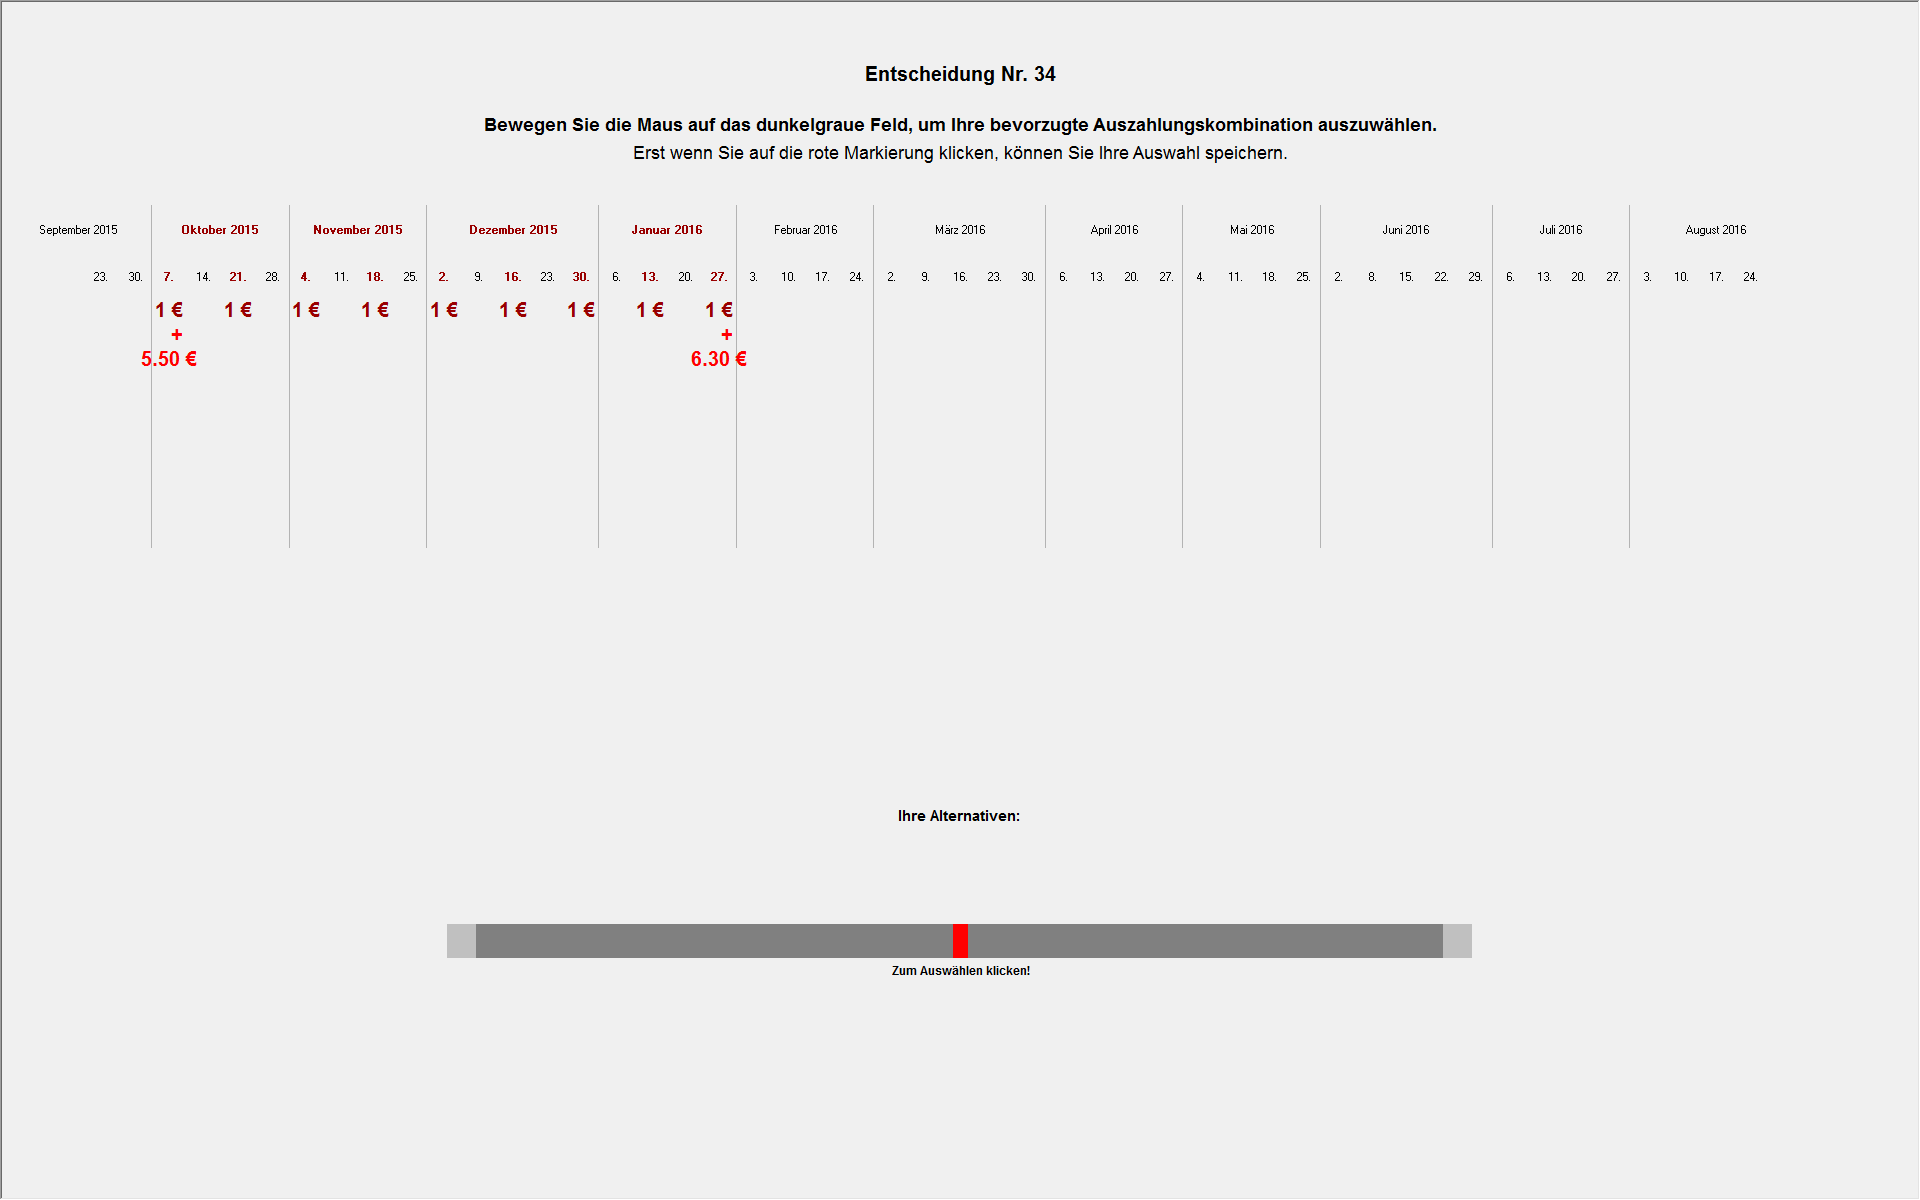
\includegraphics[width=\textwidth]{../Images/Screenshots/BS_inc_conc_half.png} \\[\medskipamount]
	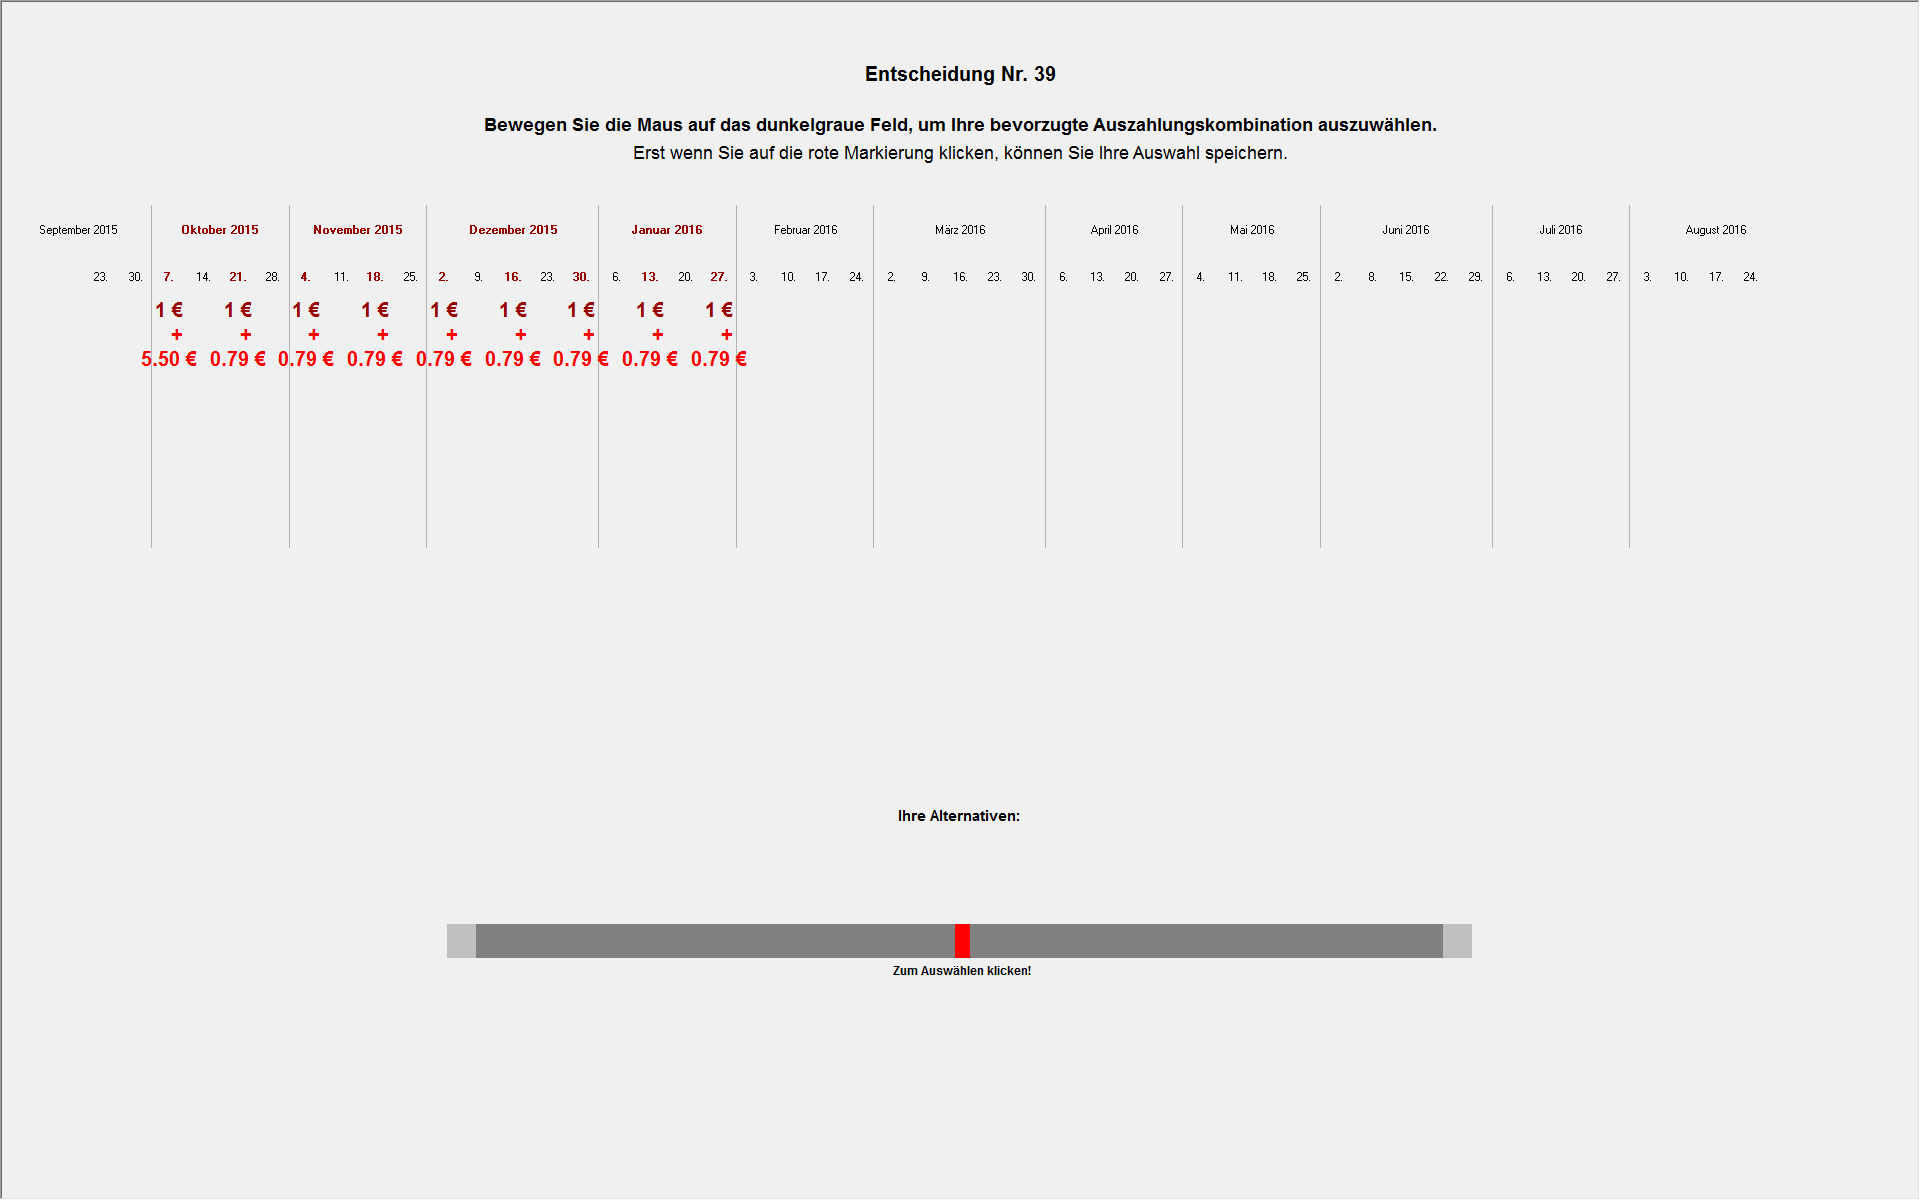
\includegraphics[width=\textwidth]{../Images/Screenshots/BS_inc_disp_half.png}
	\caption{Screenshots of a~\balA Decision (Top) and an~\unbalA[8] Decision (Bottom)%
	}
	\label{fig:screenshot:BS_inc_half}
	\begin{figurenotes}
		This figure was taken from \cite{Dertwinkel-Kalt2017}.
	\end{figurenotes}
\end{figure}%

\autoref{fig:screenshot:BS_inc_half} shows an~exemplary decision screen with ${B = \euro 11}$ and ${r \approx 15\%}$ for both \balA (upper panel) and \unbalA[8] (lower panel). Through a~slider, subjects choose their preferred ${x \in \CS[X]}$.\footnote{The slider had no initial position---it appeared only after subjects first positioned the mouse cursor over the slider bar. This was done to avoid default effects.} The slider position in Figure \ref{fig:screenshot:BS_inc_half} indicates ${x = 0.5}$, i.e., the earliest payment is reduced by \euro 5.50. Since ${r \approx 15\%}$ in this example, this slider position amounts to \euro 6.30 that are paid at later payment dates. While these \euro 6.30 are paid in a~single bank transfer on the latest payment date in \balA, the amount is dispersed in equal parts over the last 8~payment dates in \unbalA[8]---i.e., 8~consecutive payments of \euro 0.79.\footnote{We always rounded the second decimal place up so that the sum of the payments included in a~dispersed payoff was always at least as great as the respective concentrated payoff.}

\subsubsection{Some More Details}
\blindtext

Here's a~bulleted list:
\Blindlist{itemize}[3]

\subsubsection{Procedure}
\label{sec:Procedure}
Describe the sequence of events in your study. You could do this with the help of an~enumerated list:
\Blindlist{enumerate}[3]